\documentclass[a4paper, 12pt]{article}
\usepackage[margin=1in]{geometry}
\usepackage[english]{babel}
\usepackage[utf8]{inputenc}
\usepackage{tcolorbox}
\usepackage{listings}
\usepackage{color, soul}
\usepackage{xcolor}
\usepackage{amsmath}
\usepackage{mathtools}
\usepackage{graphicx}
\usepackage{textcomp}
\usepackage{url}
\tcbuselibrary{breakable}

%% MATLAB
\definecolor{codegreen}{rgb}{0,0.6,0}
\definecolor{codegray}{rgb}{0.5,0.5,0.5}
\definecolor{codepurple}{rgb}{0.58,0,0.82}
\definecolor{backcolour}{rgb}{0.95,0.95,0.92}

\lstdefinestyle{mystyle}{
	backgroundcolor = \color{backcolour},
	commentstyle = \color{codegreen},
	keywordstyle = \color{magenta},
	numberstyle = \tiny\color{codegray},
	stringstyle=\color{codepurple},
	basicstyle=\ttfamily\footnotesize,
	breakatwhitespace=false,
	breaklines=true,
	captionpos = b,
	keepspaces = true,
	numbers = left,
	numbersep = 5pt,
	showspaces = false,
	showstringspaces = false,
	showtabs = false,
	tabsize = 2
}

\lstset{style=mystyle}

%%%

\begin{document}
\title{BRI509: Introduction to Brain Signal Processing \\ Assignment No. 2}
\author{\underline{\textbf{CANOY RAYMART JAY}} \\ Student ID \#: \underline{\textbf{2020021376}}}
\date{\today}
\maketitle

\begin{itemize}
\item[\textbf{1.}]{\textbf{Explain the following terms.}}
\begin{itemize}
\item[(a)]{Impulse response}\\
\textcolor{red}{\textbf{Meaning}:} \\
The impulse response is the system's response to a unit impulse occurring at $t = 0$. If the input signal is $x(t) = \delta(t)$, then the impulse response is $y(t) = h(t)$.\\
\vspace{0.0001cm} \\
\noindent\textcolor{red}{\textbf{Convolution}}\\
The response of a system to an arbitrary input signal $x(t)$ can be calculated by convolving the input signal with the impulse response, that is, $y(t) = x(t)*h(t)$.
\begin{figure}[h!]
\center{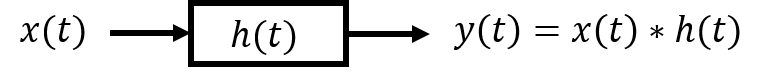
\includegraphics[width=12cm]{prob1a_convolution.png}}
\end{figure}
\begin{figure}[h!]
\center{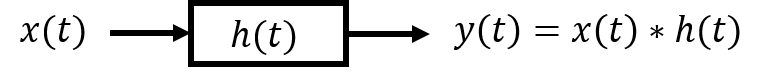
\includegraphics[width=12cm]{prob1a_convolution.png}}
\end{figure} \\
\noindent\textcolor{red}{\textbf{CTFT}}\\
In the Fourier-domain, the response of a system to an arbitrary input signal $x(t)$ can be calculated by taking the inverse Fourier transform of the product of the Fourier transforms of the input signal and the impulse response, that is, $y(t) = \mathcal{F}^{-1}\{Y(f)\} = \mathcal{F}^{-1}\{X(f)H(f)\}$.
\begin{figure}[h!]
\center{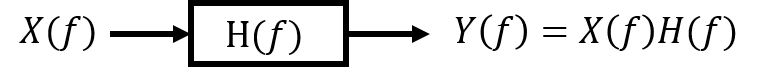
\includegraphics[width=12cm]{prob1a_CTFT.png}}
\end{figure}

\pagebreak
\item[(b)]{Harmonic functions in Fourier series}
\begin{tcolorbox}
The Fourier series of $x(t)$ is given by
\begin{equation}
x(t) = \sum_{k=0}^{+\infty}{c_{x}[k] e^{\frac{j2\pi k t}{T}}},
\end{equation}
where $k = [0, +\infty)$ is the harmonic number, $T$ is the period, and $c_{x}[k]$ is the harmonic function. The \textcolor{red}{\textbf{harmonic function}} can be represented as 
\begin{equation}
c_{x}[k] = \frac{1}{T} \int_{t_{0}}^{t_{0}+T}{x(t)e^{\frac{-j2\pi k t}{T}}} dt,
\end{equation}
where $t_{0}$ is any arbitrary time.
\end{tcolorbox}

\item[(c)]{Unit-sync function}
\begin{tcolorbox}
\begin{equation}
\mathtt{sinc} (t) = \frac{\sin(\pi t)}{\pi t}
\end{equation}
\end{tcolorbox}

\item[(d)]{How to approximate CTFT using DFT}
\begin{tcolorbox}
CTFT can be approximated at discrete frequencies by
\begin{equation}
\begin{gathered}
\begin{alignedat}{1}
X(kf_{s}/N) & \cong T_{s}\sum_{n=0}^{N-1}x(nT_{s})e^{-j2\pi kn/N} \\
& \cong T_{s} \times \mathcal{DFT}(x(nT_{s})), \; \; \; |k| << N
\end{alignedat}
\end{gathered}
\end{equation}
where $T_{s} = 1/f_{s}$ is chosen such that the signal $x(t)$ does not change much with this amount of time, and $N$ is chosen such that the signal energy of the signal $x(t)$ can be covered within the time range $0$ to $NT_{s}$.
\end{tcolorbox}

\item[(e)]{Graph the CTFT of cosine function $\cos ( 2\pi f_{0} t)$ and sine function $\sin ( 2 \pi f_{0} t)$}
\begin{equation}
\begin{gathered}
\begin{alignedat}{1}
\cos(2 \pi f_{0}t) \overset{\mathcal{F}}{\leftrightarrow} \frac{1}{2} \left[ \delta(f - f_{0}) + \delta (f+ f_{0})\right]
\end{alignedat}
\end{gathered}
\end{equation}

\begin{figure}[h!]
\center{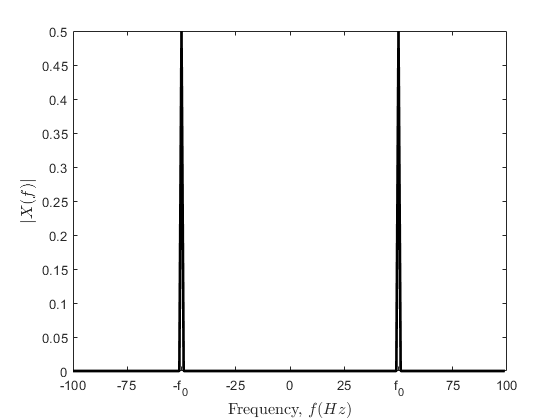
\includegraphics[width=5cm]{prob1e_cosine.png}}
\caption{The CTFT of $\cos (2 \pi f_{0} t)$}
\end{figure}

\begin{equation}
\begin{gathered}
\begin{alignedat}{1}
\sin(2 \pi f_{0}t) \overset{\mathcal{F}}{\leftrightarrow} \frac{j}{2} \left[ \delta(f + f_{0}) - \delta (f- f_{0})\right]
\end{alignedat}
\end{gathered}
\end{equation}

\begin{figure}[h!]
\center{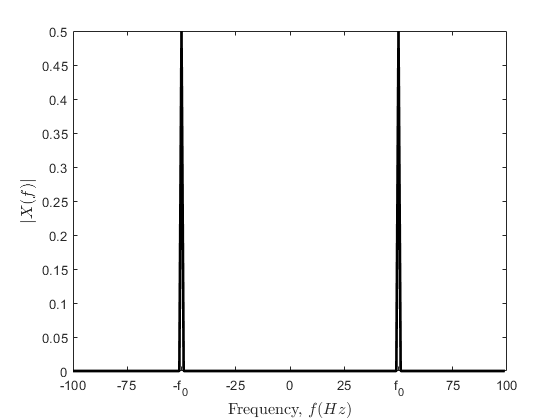
\includegraphics[width=5cm]{prob1e_sine.png}}
\caption{The CTFT of $\sin (2 \pi f_{0} t)$}
\end{figure}
\end{itemize}

\item[\textbf{2.}]{\textbf{Solve the following problems.}}
\begin{itemize}
\item[(a)]{Find the impulse response $h[n]$ of the system described by the difference equation}
\begin{equation}
5y[n] + 2y[n-1] - 3y[n-2] = x[n]
\end{equation}

\textcolor{red}{\textbf{Solution:}}
\begin{itemize}
\item[(i)]{Let $x[n] = \delta[n] \; \; \; \rightarrow \; \; \; y[n] = h[n]$. The difference equation now becomes}
\begin{equation}
5h[n] + 2h[n-1] - 3h[n-2] = \delta[n].
\label{eq:2a_difference_equation}
\end{equation}
\item[(ii)]{\textcolor{red}{Homogeneous Solution:}}
\begin{itemize}
\item[(1.)]{Let $h[n] = K_{h}z^{n}$.}
\item[(2.)]{Substituting this into the difference equation will give}
\begin{equation}
\begin{gathered}
\begin{alignedat}{1}
5h[n] + 2h[n-1] - 3h[n-2] &= 0 \\
5K_{h}z^{n} + 2K_{h}z^{n-1} - 3 K_{h}z^{n-2} &= 0 \\
K_{h}z^{n-2} \left( 5z^{2} + 2z - 3 \right) &= 0 \\
5z^{2} + 2z - 3 &= 0 \\
z_{1,2} &= \frac{-2 \pm \sqrt{4 - 4(5)(-3)}}{2(5)} \\
\Aboxed{z_{1} = \frac{-2 + 8}{10} = \frac{3}{5}} \Aboxed{z_{2} = \frac{-2 - 8}{10} = -1}
\end{alignedat}
\end{gathered}
\end{equation}
\item[(3.)]{Therefore, the impulse response can now be represented as}
\begin{equation}
h[n] = K_{h, 1} \left(\frac{3}{5} \right)^{n} + K_{h, 2} \left(-1 \right)^{n}
\end{equation}
\item[(4.)]{Initial conditions:} \\
\begin{center}
\begin{tabular}{|c |c | c | c |c|}
\hline
$n$ & $x[n]$ & $y[n-2]$ & $y[n-1]$ & $y[n]$ \\
\hline
0 & $x[0] = 1$ & $h[-2] = 0$ & $h[-1] = 0$ & $5h[0] + 2h[-1] - 3 h[-2] = 1$ \\
& & & & $h[0] = \frac{1}{5}$ \\
\hline
1 & $x[1] = 0$ & $h[-1] = 0$ & $h[0] = \frac{1}{5}$ & $5h[1] + 2h[0] - 3h[-1] = 0$ \\
& & & & $h[1] = \frac{-2}{25}$ \\
\hline
\end{tabular}
\end{center}
\item[(5.)]{Applying the initial conditions:} \\
\textcolor{red}{Initial Condition 1:}
\begin{equation}
\begin{gathered}
\begin{alignedat}{1}
h[0] = \frac{1}{5} &= K_{h, 1} \left( \frac{3}{5}\right)^{0} + K_{h, 2}\left(-1 \right)^{0} \\
\frac{1}{5} &= K_{h, 1} + K_{h, 2}
\end{alignedat}
\end{gathered}
\end{equation}
\textcolor{red}{Initial Condition 2:}
\begin{equation}
\begin{gathered}
\begin{alignedat}{1}
h[1] = \frac{-2}{25} & = K_{h,1} \left(\frac{3}{5} \right)^{1} + K_{h,2} \left(-1 \right)^{1} \\
\frac{-2}{25} &= K_{h,1} \left(\frac{3}{5} \right) + K_{h,2}(-1)
\end{alignedat}
\end{gathered}
\end{equation}
These system of equations can be written in matrix form as
\begin{center}
\begin{equation}
\begin{gathered}
\begin{alignedat}{1}
\begin{bmatrix}
\frac{1}{5} \\
\frac{-2}{25}
\end{bmatrix} &= 
\begin{bmatrix}
1 & 1 \\
\frac{3}{5} & -1
\end{bmatrix}
\begin{bmatrix}
K_{h,1} \\
K_{h,2}
\end{bmatrix} \\
\begin{bmatrix}
K_{h, 1} \\
K_{h, 2}
\end{bmatrix} &=
\begin{bmatrix}
1 & 1 \\
\frac{3}{5} & -1
\end{bmatrix}^{-1} 
\begin{bmatrix}
\frac{1}{5} \\
\frac{-2}{25}
\end{bmatrix} \\
\begin{bmatrix}
K_{h, 1} \\
K_{h, 2}
\end{bmatrix} &=
\begin{bmatrix}
\frac{3}{40} \\
\frac{5}{40}
\end{bmatrix}
\end{alignedat}
\end{gathered}
\end{equation}
\end{center}
\end{itemize}
\item[(iii.)]{Therefore, the impulse response is given by}
\begin{equation}
\boxed{h[n] = \frac{3}{40} \left(\frac{3}{5} \right)^{n} + \frac{5}{40} \left(-1 \right)^{n}}
\end{equation}
\end{itemize}

\pagebreak
\item[(b)]{Find the convolution of the two functions $x_{1}(t)$ and $x_{2}(t)$.}
\begin{figure}[h!]
\center{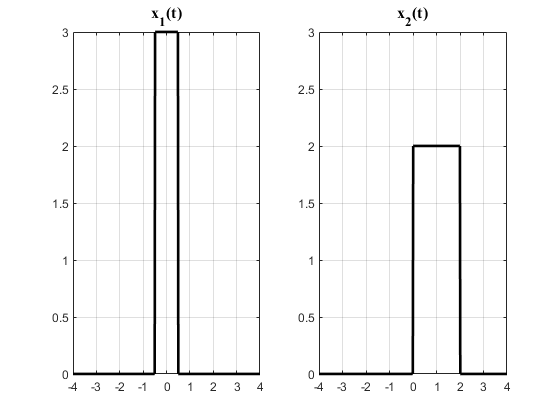
\includegraphics[width=12cm,]{Prob2b_problem_statement.png}}
\end{figure} \\
\textcolor{red}{\textbf{Solution}}
\begin{itemize}
\item[(i.)]{The functions $x_{1}(t)$ and $x_{2}(t)$ can be represented as}
\begin{equation}
x_{1}(t) = 3\mathtt{rect}(t) = 3 \left[ \mathtt{u}\left(t + \frac{1}{2}\right) - \mathtt{u}\left(t - \frac{1}{2}\right)\right]
\end{equation}

\begin{equation}
\begin{gathered}
\begin{alignedat}{1}
x_{2}(t) = 2\mathtt{rect}\left(\frac{t-1}{2}\right) &= 2\left[\mathtt{u}\left(\frac{t}{2} \right) - \mathtt{u}\left(\frac{t - 2}{2} \right) \right] \\
&= 2\left[\mathtt{u}\left(t \right) - \mathtt{u}\left(t-2 \right) \right] 
\end{alignedat}
\end{gathered}
\end{equation}

\item[(ii.)]{From the differentiation property of convolution, $y^{'}(t) = x^{'}(t)*h(t)$ or $y^{'}(t) = x(t)*h^{'}(t)$. Therefore,}
\begin{equation}
\begin{gathered}
\begin{alignedat}{1}
y(t) &= x_{1}(t) * x_{2}(t) \\ 
y^{'}(t) &= x_{1}^{'}(t) * x_{2}(t) \\
y^{''}(t) &= x_{1}^{'}(t) * x_{2}^{'}(t) \\
y^{''}(t) &= 2\left[\delta \left( t + \frac{1}{2}\right) - \delta \left(t - \frac{1}{2} \right) \right] * 3 \left[\delta \left( t\right) - \delta \left( t - 2 \right)\right] \\
y^{''}(t) &= 6\Biggr[\delta\left( t + \frac{1}{2}\right) * \delta(t) - \delta \left(t + \frac{1}{2} \right) * \delta(t -2) - \delta\left(t - \frac{1}{2} \right)*\delta(t)\\
&+ \delta\left(t - \frac{1}{2} \right)*\delta(t-2) \Biggr] \\
\end{alignedat}
\end{gathered}
\end{equation}

\begin{equation}
\begin{gathered}
\begin{alignedat}{1}
y^{''}(t) &= 6\left[ \delta \left(t + \frac{1}{2} \right) - \delta \left(t - \frac{3}{2} \right) - \delta\left( t - \frac{1}{2}\right) + \delta \left(t - \frac{5}{2} \right) \right] \\
y^{'}(t) &= 6\left[ \mathtt{u} \left(t + \frac{1}{2} \right) - \mathtt{u} \left(t - \frac{3}{2} \right) - \mathtt{u}\left( t - \frac{1}{2}\right) + \mathtt{u} \left(t - \frac{5}{2} \right) \right] \\
\Aboxed{y(t) &= 6\left[ \mathtt{ramp} \left(t + \frac{1}{2} \right) - \mathtt{ramp} \left(t - \frac{3}{2} \right) - \mathtt{ramp}\left( t - \frac{1}{2}\right) + \mathtt{ramp} \left(t - \frac{5}{2} \right) \right]}
\end{alignedat}
\end{gathered}
\end{equation}
\item[(iii.)]{Table of values}
\begin{center}
\begin{tabular}{|c|c|}
\hline
$t$ & $y(t)$ \\
\hline
$t = \frac{-1}{2}$ & $y\left(\frac{-1}{2}\right) = 6 \left(0 - 0 -0 + 0\right) = 0$\\
\hline
$t = 0$ & $y\left(0\right) = 6 \left(\frac{1}{2} - 0 -0 + 0\right) = 3$ \\
\hline
$t = \frac{1}{2}$ & $y\left(\frac{1}{2}\right) = 6 \left(1 - 0 -0 + 0\right) = 6$ \\
\hline
$t = 1$ & $y\left(1\right) = 6 \left(\frac{3}{2} - 0 -\frac{1}{2} + 0\right) = 6$ \\
\hline
$t = \frac{3}{2}$ & $y\left(\frac{3}{2}\right) = 6 \left(2 - 0 -1 + 0\right) = 6$ \\
\hline
$t = 2$ & $y\left(2\right) = 6 \left(\frac{5}{2} - \frac{1}{2} -\frac{3}{2} + 0\right) = 3$ \\
\hline
$t = \frac{5}{2}$ & $y\left(\frac{5}{2}\right) = 6 \left(3 - 1 -2 + 0\right) = 0$ \\
\hline
\end{tabular}
\end{center}
\item[(iv.)]{Plot of the convolution of $x_{1}(t)$ and $x_{2}(t)$:}
\begin{figure}[h!]
\center{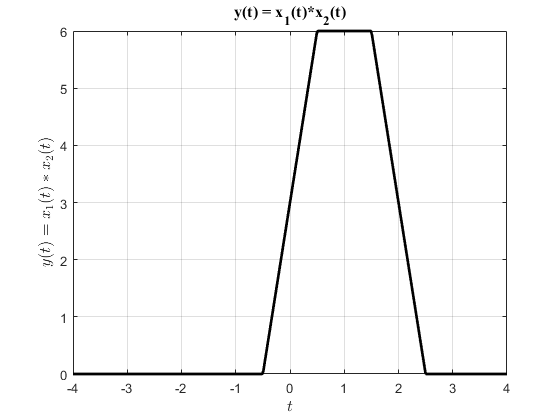
\includegraphics[width=12cm]{Prob_2b_convolution.png}}
\caption{\label{fig:2b_convolution}Plot of the convolution of $x_{1}(t) = 3\mathtt{rect}(t)$ and $x_{2}(t)= 2\mathtt{rect}(\frac{t-1}{2})$}
\end{figure}
\end{itemize}

\pagebreak
\item[(c)]{Find the complex CTFS harmonic function of $x(t) = 10\mathtt{rect}(t/2)*\delta_{4}(t)$ using}
\begin{equation}
c_{x}[k] = \frac{1}{T}\int_{T}{x(t)e^{\frac{-j2\pi kt}{T}}} dt
\end{equation}

\textcolor{red}{\textbf{Solution}}
\begin{itemize}
\item[(i.)]{From $x(t) = 10\mathtt{rect}(t/2)*\delta_{\mathbf{T}}(t) = 10\mathtt{rect}(t/2)*\delta_{4}(t)$, the period can be written as $T = 4$. Also, the width of the rectangle function $\mathtt{rect}(t/2)$ is $w = 2$.}
\item[(ii.)]{Thus, the harmonic function can be calculated as:}
\begin{equation}
\begin{gathered}
\begin{alignedat}{1}
c_{x}[k] &= \frac{1}{T}\int_{T}{x(t)e^{\frac{-j2\pi k t}{T}}} dt\\
&= \frac{1}{T}\int_{-T/2}^{T/2}{10\mathtt{rect}(t/2)*\delta_{4}(t)e^{\frac{-j2\pi k t}{T}}} dt \\
&= \frac{10}{4}\int_{-4/2}^{4/2}{\mathtt{rect}(t/2)} e^{\frac{-j2\pi k t}{4}}dt \\
&= \frac{5}{2}\int_{-1}^{1}{e^{\frac{-j2\pi k t}{4}}} dt\\
&= \frac{5}{2}\Biggr( \frac{e^{\frac{-j2\pi k t}{4}}}{-j2 \pi k/4} \Biggr|^{1}_{-1} \\
&= \frac{5}{2} \Biggr( \frac{e^{-j2 \pi k / 4} - e^{j2 \pi k / 4}}{-j2 \pi k/4} \Biggr) \\
&= \frac{5}{2} \left( \frac{\sin\left(2 \pi k /4 \right)}{\pi k/ 4}\right) = \frac{5}{2} \left( \frac{\sin\left( \pi k /2 \right)}{\pi k/ 4}\right) \cdot \frac{2}{2} \\
&= 5 \left(\frac{\sin\left(\pi k /2 \right)}{\pi k/2} \right) \\
\Aboxed{c_{x}[k]&= 5 \mathtt{sinc(k/2)}\cdot \delta_{1}[k]}
\end{alignedat}
\end{gathered}
\end{equation}
\end{itemize}

\pagebreak
\item[(d)]{Find the CTFT of $x_{t} = 24\cos\left(100\pi t \right) \sin \left(10,000 \pi t \right)$.}
\begin{figure}[h!]
\center{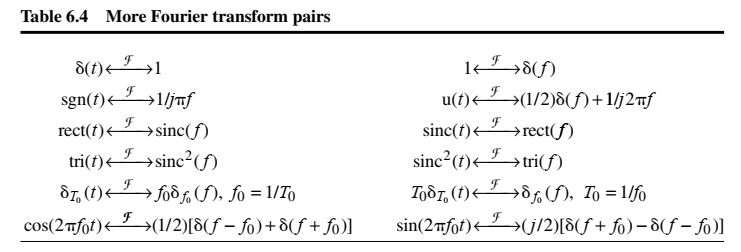
\includegraphics[width=12cm]{Prob2d_Fourier_transform_pairs.png}}
\end{figure} \\
\textcolor{red}{\textbf{Solution}}
\begin{itemize}
\item[(i.)]{$\cos \left(2 \pi f_{0} t\right) \overset{\mathcal{F}}{\leftrightarrow} \frac{1}{2} \left[\delta \left(f - f_{0}\right) + \delta(f + f_{0}) \right]$. Therefore,}
\begin{equation}
\begin{gathered}
\begin{alignedat}{1}
24 \cos \left(100 \pi t \right) \overset{\mathcal{F}}{\leftrightarrow} &\frac{24}{2} \left[ \delta \left(f - 50 \right) + \delta \left(f + 50 \right) \right] \\
& = 12 \left[ \delta \left(f - 50\right) + \delta \left(f + 50 \right) \right]
\end{alignedat}
\end{gathered}
\end{equation}
\item[(ii.)]{$\sin \left(2 \pi f_{0} t\right) \overset{\mathcal{F}}{\leftrightarrow} \frac{1}{2} \left[\delta \left(f + f_{0}\right) - \delta(f - f_{0}) \right]$. Therefore,}
\begin{equation}
\sin \left(10,000 \pi t \right) \overset{\mathcal{F}}{\leftrightarrow}  \frac{j}{2}\left[ \delta \left(f + 5,000 \right) - \delta \left(f - 5,000 \right) \right]
\end{equation}
\item[(iii.)]{$g(t)h(t) \overset{\mathcal{F}}{\leftrightarrow} G(f)*H(f)$. Therefore,}
\begin{equation}
\begin{gathered}
\begin{alignedat}{1}
24 \cos \left(100 \pi t \right) \sin \left(10,000 \pi t \right) \overset{\mathcal{F}}{\leftrightarrow} & 12 \left[ \delta \left(f - 50\right) + \delta \left(f + 50 \right) \right] * \frac{j}{2}[ \delta \left(f + 5,000 \right) \\
&\;\;\;\;\;- \delta \left(f - 5,000 \right)] \\
& = j6 [ \delta \left(f - 50\right) * \delta \left(f + 5,000 \right) \\
& \;\;\;\;\;\;\;\;\; - \delta \left(f - 50\right) * \delta \left(f - 5,000 \right) \\
& \;\;\;\;\;\;\;\;\; + \delta \left(f + 50\right) * \delta \left(f + 5,000 \right) \\
& \;\;\;\;\;\;\;\;\; - \delta \left(f + 50\right) * \delta \left(f - 5,000 \right)] \\
24 \cos \left(100 \pi t \right) \sin \left(10,000 \pi t \right) \overset{\mathcal{F}}{\leftrightarrow} & \;\;\;\;\; j6 [ \delta(f + 4950) - \delta (f - 5050) \\
& \;\;\;\;\;\;\;\;\;+ \delta ( f + 5050) - \delta(f - 4950)]
\end{alignedat}
\end{gathered}
\end{equation}
\end{itemize}

\pagebreak
\item[(e)]{Find and graph the inverse DTFT of}
\begin{equation}
X(F) = \left[\mathtt{rect}\left(50\left( F-\frac{1}{4}\right) \right) + \mathtt{rect}\left(50\left( F+\frac{1}{4}\right) \right)\right]*\delta_{1}(F)
\end{equation}
\begin{figure}[h!]
\center{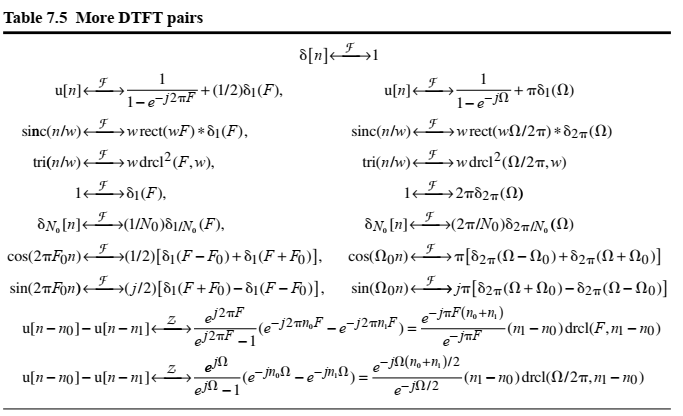
\includegraphics[width=12cm]{Prob2e_DTFT_pairs.png}}
\end{figure} \\
\textcolor{red}{\textbf{Solution}}
\begin{itemize}
\item[(i.)]{$\mathtt{sinc}\left(\frac{n}{w} \right) \overset{\mathcal{F}}{\leftrightarrow} w\mathtt{rect}\left(wF \right) * \delta_{1}(F)$. Therefore, if $w=50$, then}
\begin{equation}
\begin{gathered}
\begin{alignedat}{1}
\frac{1}{50} \mathtt{sinc} \left(\frac{n}{50} \right) &\overset{\mathcal{F}}{\leftrightarrow} \frac{1}{50} \cdot 50 \mathtt{rect} \left(50F \right)*\delta_{1}(F) = \mathtt{rect}(50F)*\delta_{1}(F)
\end{alignedat}
\end{gathered}
\end{equation}
\item[(ii.)]{The frequency shifting property is given by $e^{j2\pi F_{0} n} x[n] \overset{\mathcal{F}}{\leftrightarrow} X(F - F_{0})$. Therefore,}\\
$F_{0} = \frac{1}{4}$:
\begin{equation}
\begin{gathered}
\begin{alignedat}{1}
e^{j2\pi n/4} \cdot \frac{1}{50} \mathtt{sinc} \left(\frac{n}{50} \right) \overset{\mathcal{F}}{\leftrightarrow} \mathtt{rect}\left(50\left(F - \frac{1}{4}\right)\right)*\delta_{1}(F)
\end{alignedat}
\end{gathered}
\label{eq:2e_f0_1_4}
\end{equation} \\
$F_{0} = -\frac{1}{4}$:
\begin{equation}
\begin{gathered}
\begin{alignedat}{1}
e^{-j2\pi n/4} \cdot \frac{1}{50} \mathtt{sinc} \left(\frac{n}{50} \right) \overset{\mathcal{F}}{\leftrightarrow} \mathtt{rect}\left(50\left(F + \frac{1}{4}\right)\right)*\delta_{1}(F)
\end{alignedat}
\end{gathered}
\label{eq:2e_f0__1_4}
\end{equation}
\item[(iii.)]{Adding eqs. \eqref{eq:2e_f0_1_4} and \eqref{eq:2e_f0__1_4} gives}
\begin{equation}
\begin{gathered}
\begin{alignedat}{1}
\left(e^{j2\pi n/4} +  e^{-j2\pi n/4}\right) \frac{1}{50} \mathtt{sinc} \left(\frac{n}{50} \right) \overset{\mathcal{F}}{\leftrightarrow} &\Biggr[\mathtt{rect}\left(50\left(F - \frac{1}{4}\right)\right) \\
&\;+ \mathtt{rect}\left(50\left(F + \frac{1}{4}\right)\right) \Biggr]*\delta_{1}(F)
\end{alignedat}
\end{gathered}
\end{equation}
Therefore, the inverse DTFT of
\begin{equation}
X(F) = \left[\mathtt{rect}\left(50\left(F - \frac{1}{4}\right)\right) + \mathtt{rect}\left(50\left(F + \frac{1}{4}\right)\right) \right]*\delta_{1}(F)
\end{equation}
is:
\begin{equation}
\begin{gathered}
\begin{alignedat}{1}
x[n] &= \left(e^{j2\pi n/4} +  e^{-j2\pi n/4}\right) \frac{1}{50} \mathtt{sinc} \left(\frac{n}{50} \right) \\
&= 2 \cos \left(\frac{2\pi n}{4} \right) \cdot \frac{1}{50} \mathtt{sinc} \left(\frac{n}{50} \right) \\
\Aboxed{x[n] & = \frac{1}{25} \cos \left(\frac{\pi n}{2} \right)  \mathtt{sinc} \left(\frac{n}{50} \right)}
\end{alignedat}
\end{gathered}
\end{equation}

\begin{figure}[h!]
\center{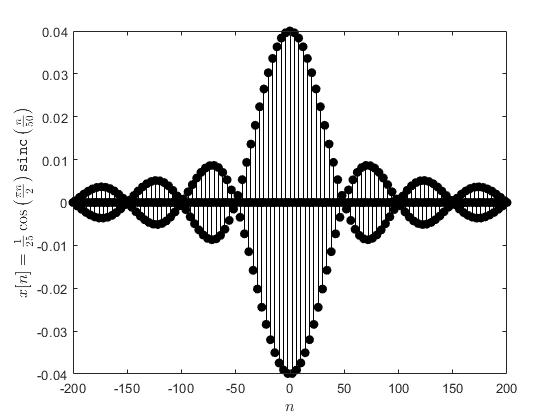
\includegraphics[width=12cm]{prob2e.png}}
\caption{\label{fig:2e}The inverse DTFT of $X(F) = \left[\mathtt{rect}\left(50\left(F - \frac{1}{4}\right)\right) + \mathtt{rect}\left(50\left(F + \frac{1}{4}\right)\right)\right]*\delta_{1}(F)$}
\end{figure}
\end{itemize}
\end{itemize}

\pagebreak
\item[\textbf{3.}]{\textbf{MATLAB coding}}
\begin{itemize}
\item[(a)]{Using the DFT, find the approximate CTFT of}
\[
x(t) = 
\begin{cases}
t(1-t), & 0 < t < 1 \\
0, & \mathtt{otherwise}
\end{cases}
\Biggr\rbrace= t(1-t)\mathtt{rect}\left(t - \frac{1}{2} \right)
\]

\begin{tcolorbox}[enforce breakable, pad at break = 1mm, break at=18cm,title={Source Code}]
\lstinputlisting[language=Matlab, upquote=true]{prob3a.m}
\end{tcolorbox}

\begin{figure}[h!]
\center{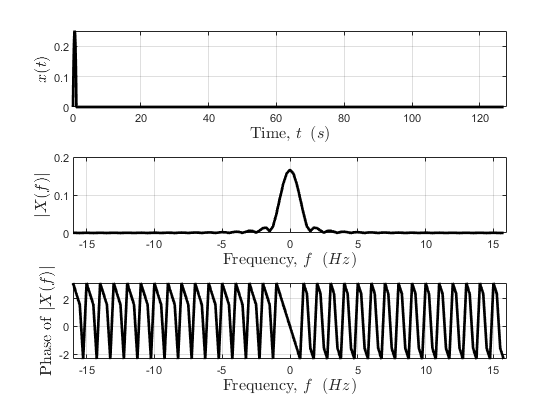
\includegraphics[width=15cm]{prob3a.png}}
\end{figure}

\pagebreak
\item[(b.1)]{Graph the CTFT of of C4(523.25/2Hz), D4 (587.33/2Hz), E4 (659.26/2Hz), F4 (698.46/2Hz), G4 (784/2Hz), A4 (440Hz), B4 (493.8Hz), C5 (523.25Hz).}

\begin{tcolorbox}[enforce breakable, pad at break = 1mm, break at=23cm,title={Source Code}]
\lstinputlisting[language=Matlab, upquote=true]{prob3b_1.m}
\end{tcolorbox}

\begin{figure}[h!]
\center{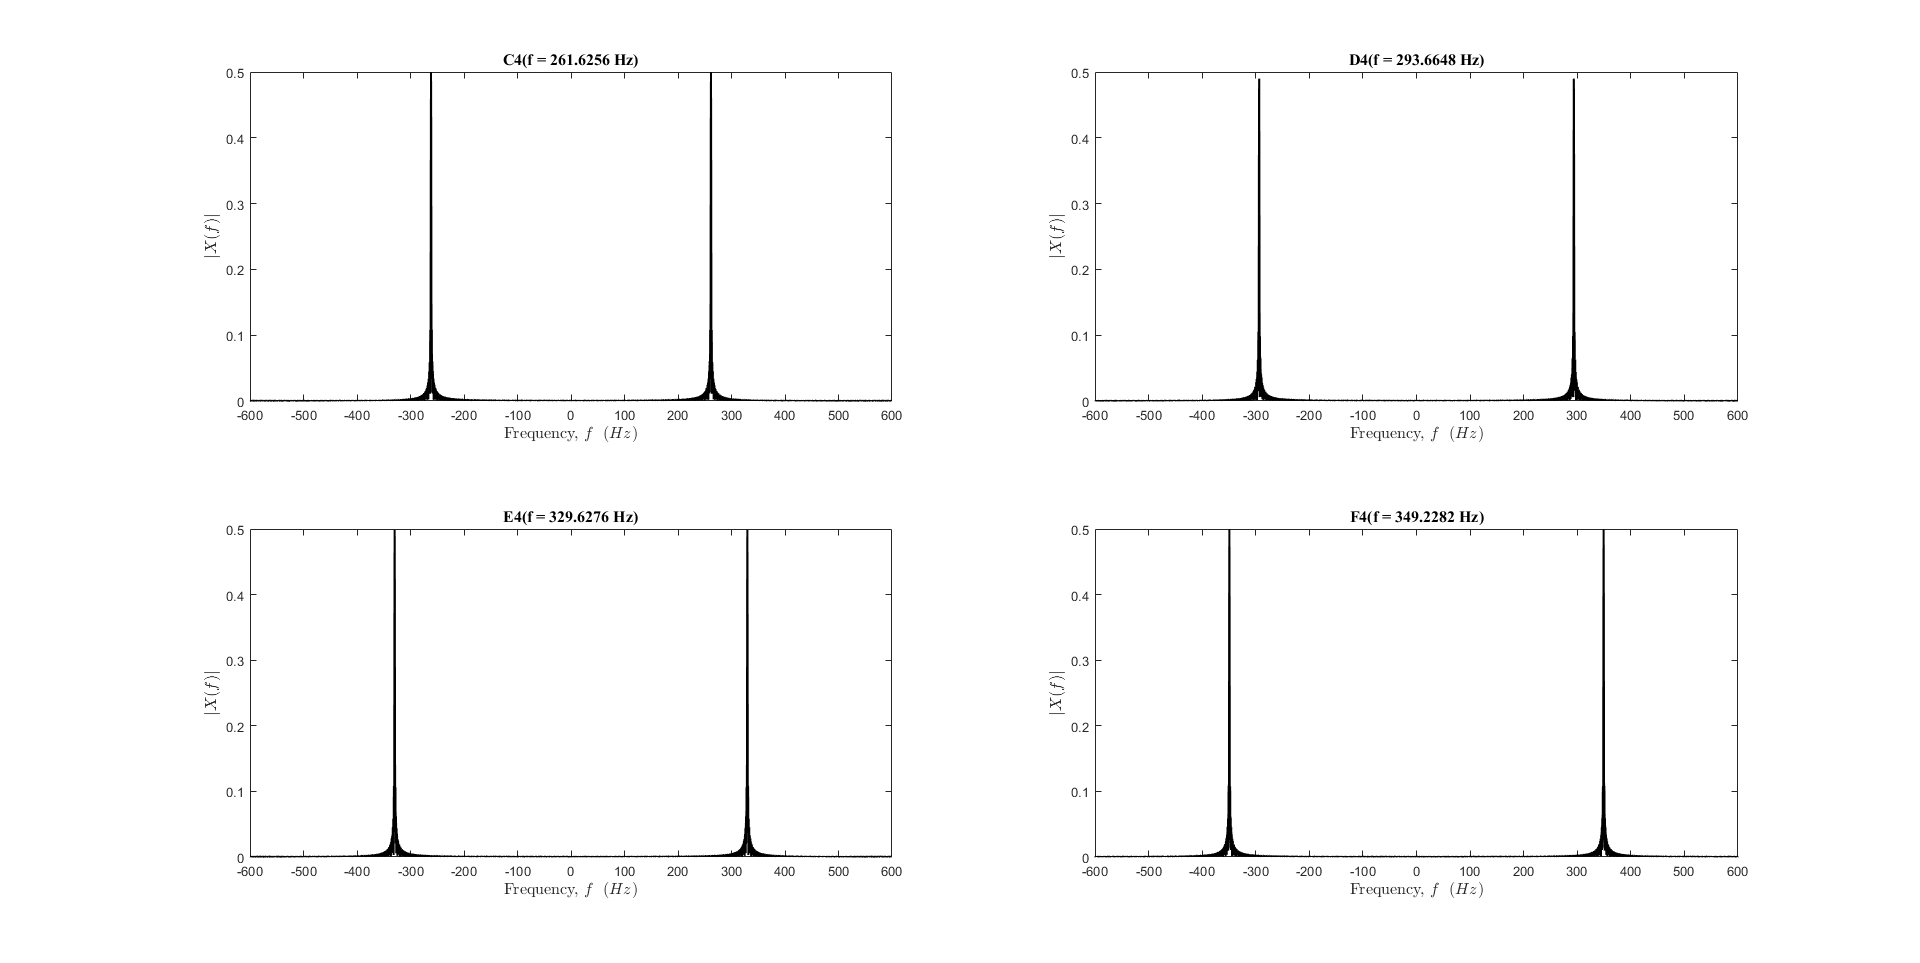
\includegraphics[width=18cm]{prob3b_1_1.png}}
\end{figure}

\begin{figure}[h!]
\center{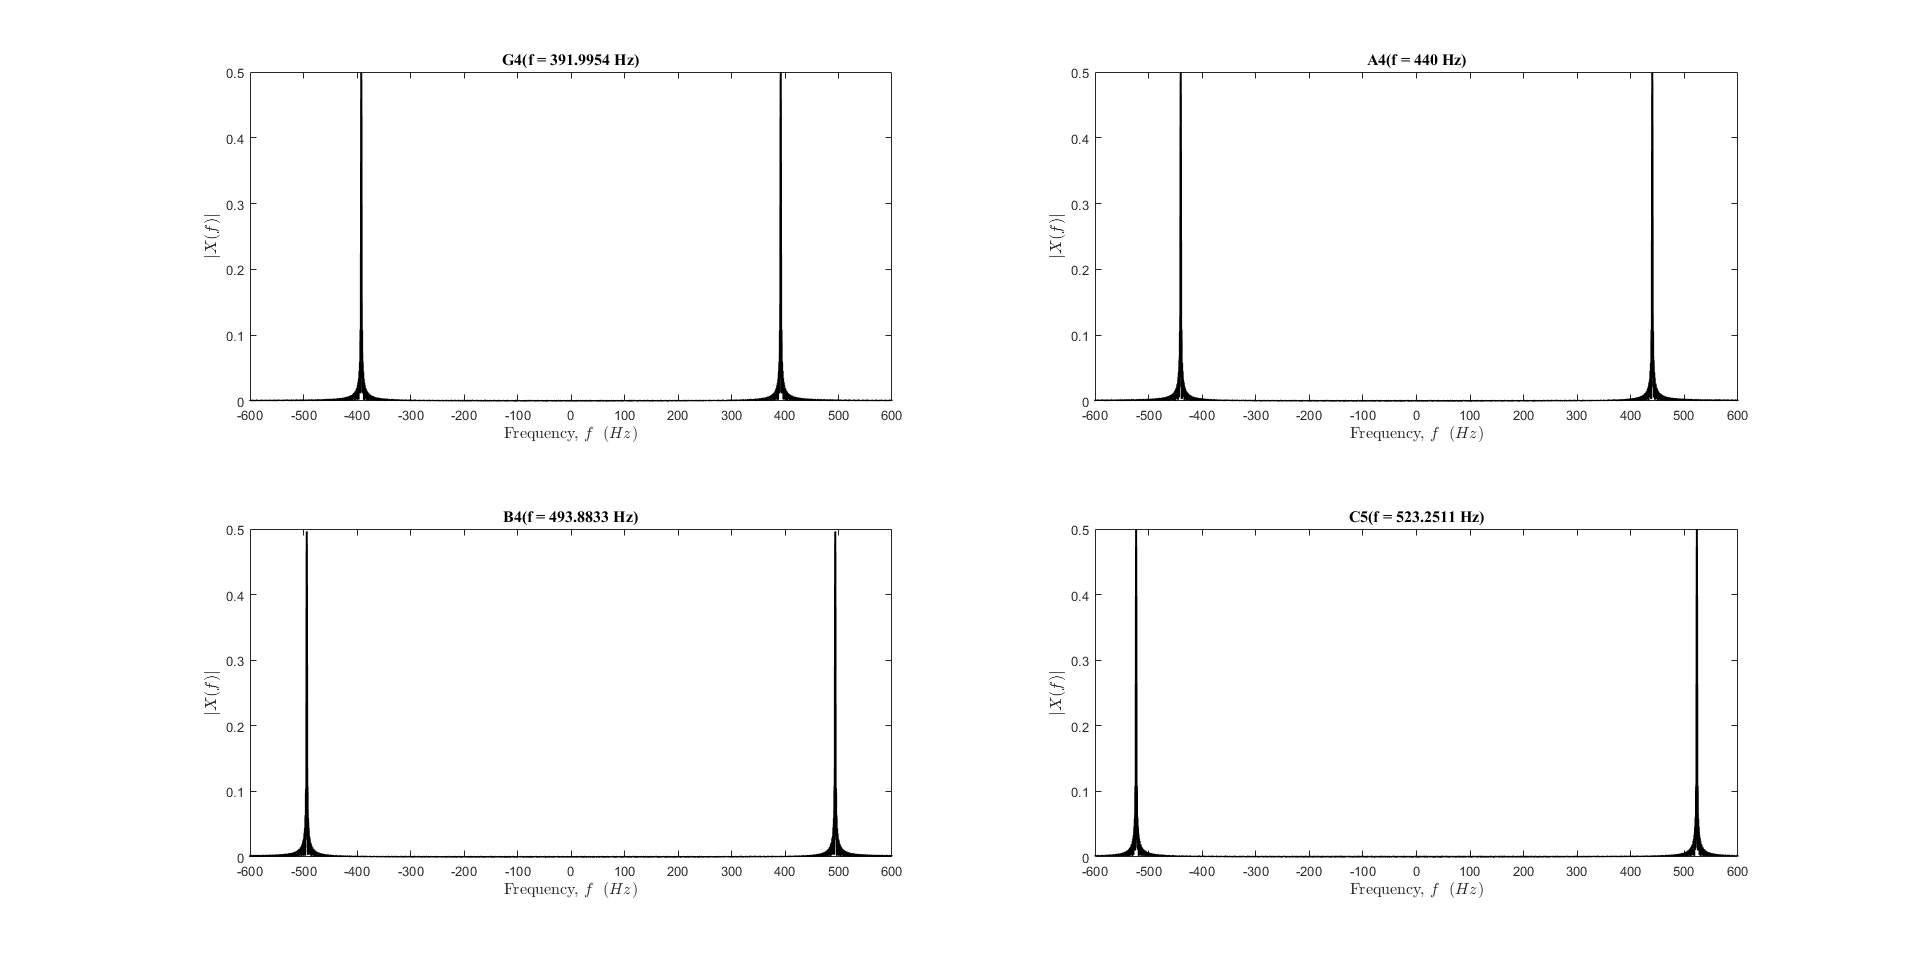
\includegraphics[width=18cm]{prob3b_1_2.png}}
\caption{\label{fig:3b}CTFT of the solfeges of C Major.}
\end{figure}

\vspace{10cm}
\pagebreak

\item[(b.2)]{Make an MP3 file containing C4, D4, E4, F4, G4, A4, B4, C5.}

\begin{tcolorbox}[enforce breakable, pad at break = 1mm, break at=23cm,title={Source Code}]
\lstinputlisting[language=Matlab, upquote=true]{prob3b_2.m}
\end{tcolorbox}

\vspace{2cm}
\begin{tcolorbox}[title={\textbf{Note: All the files were uploaded on GitHub}}]
All the files in this document were uploaded on Github, and can be accessed at:


\begin{center}
\url{https://github.com/rjcanoy03/BRI509/tree/Assignment%232}
\end{center}


If there are errors in the solution or codes kindly email, $\\$
recanoy@korea.ac.kr.
\end{tcolorbox}
\end{itemize}
\end{itemize}
\end{document}